% ------------------------------------------------
% Page start
%\newpage
%\phantomsection
% ------------------------------------------------

\chapter{各系所博碩士撰寫論文須知}
\label{appendix:thesis-spec}

\section{介紹}
這部份資料來源是使用'電機工程系辦網頁'中的'論文撰寫須知.pdf'(\url{"http://office.ee.ncku.edu.tw/uploads/\%E8\%AB\%96\%E6\%96\%87\%E6\%92\%B0\%E5\%AF\%AB\%E9\%A0\%88\%E7\%9F\%A5.pdf}).\\

但由於原檔案沒法顯示, 故需要另重新儲存成一個新的出來. 使用學校的Adobe Acrobat XI試驗, 發現要使用'儲存為其他->可存檔PDF (PDF/A)'才能顯示出來.\\

\begin{figure}[h]
\centering
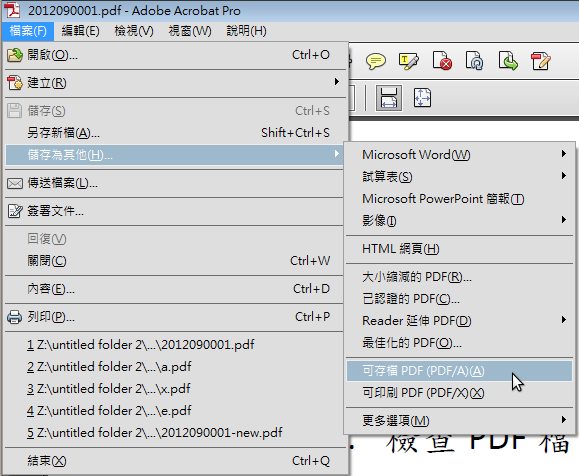
\includegraphics[scale=0.3]{./example/appendix/pic/save_pdf.png}
\caption{在Adobe Acrobat另存新版本}
\label{fig:appendix:save_pdf}
\end{figure}

檔案位置:\\
新: 'example/appendix/pdf/thesis-spec.pdf'\\
原: 'example/appendix/pdf/論文撰寫須知.pdf'\\

\setboolean{@twoside}{false}
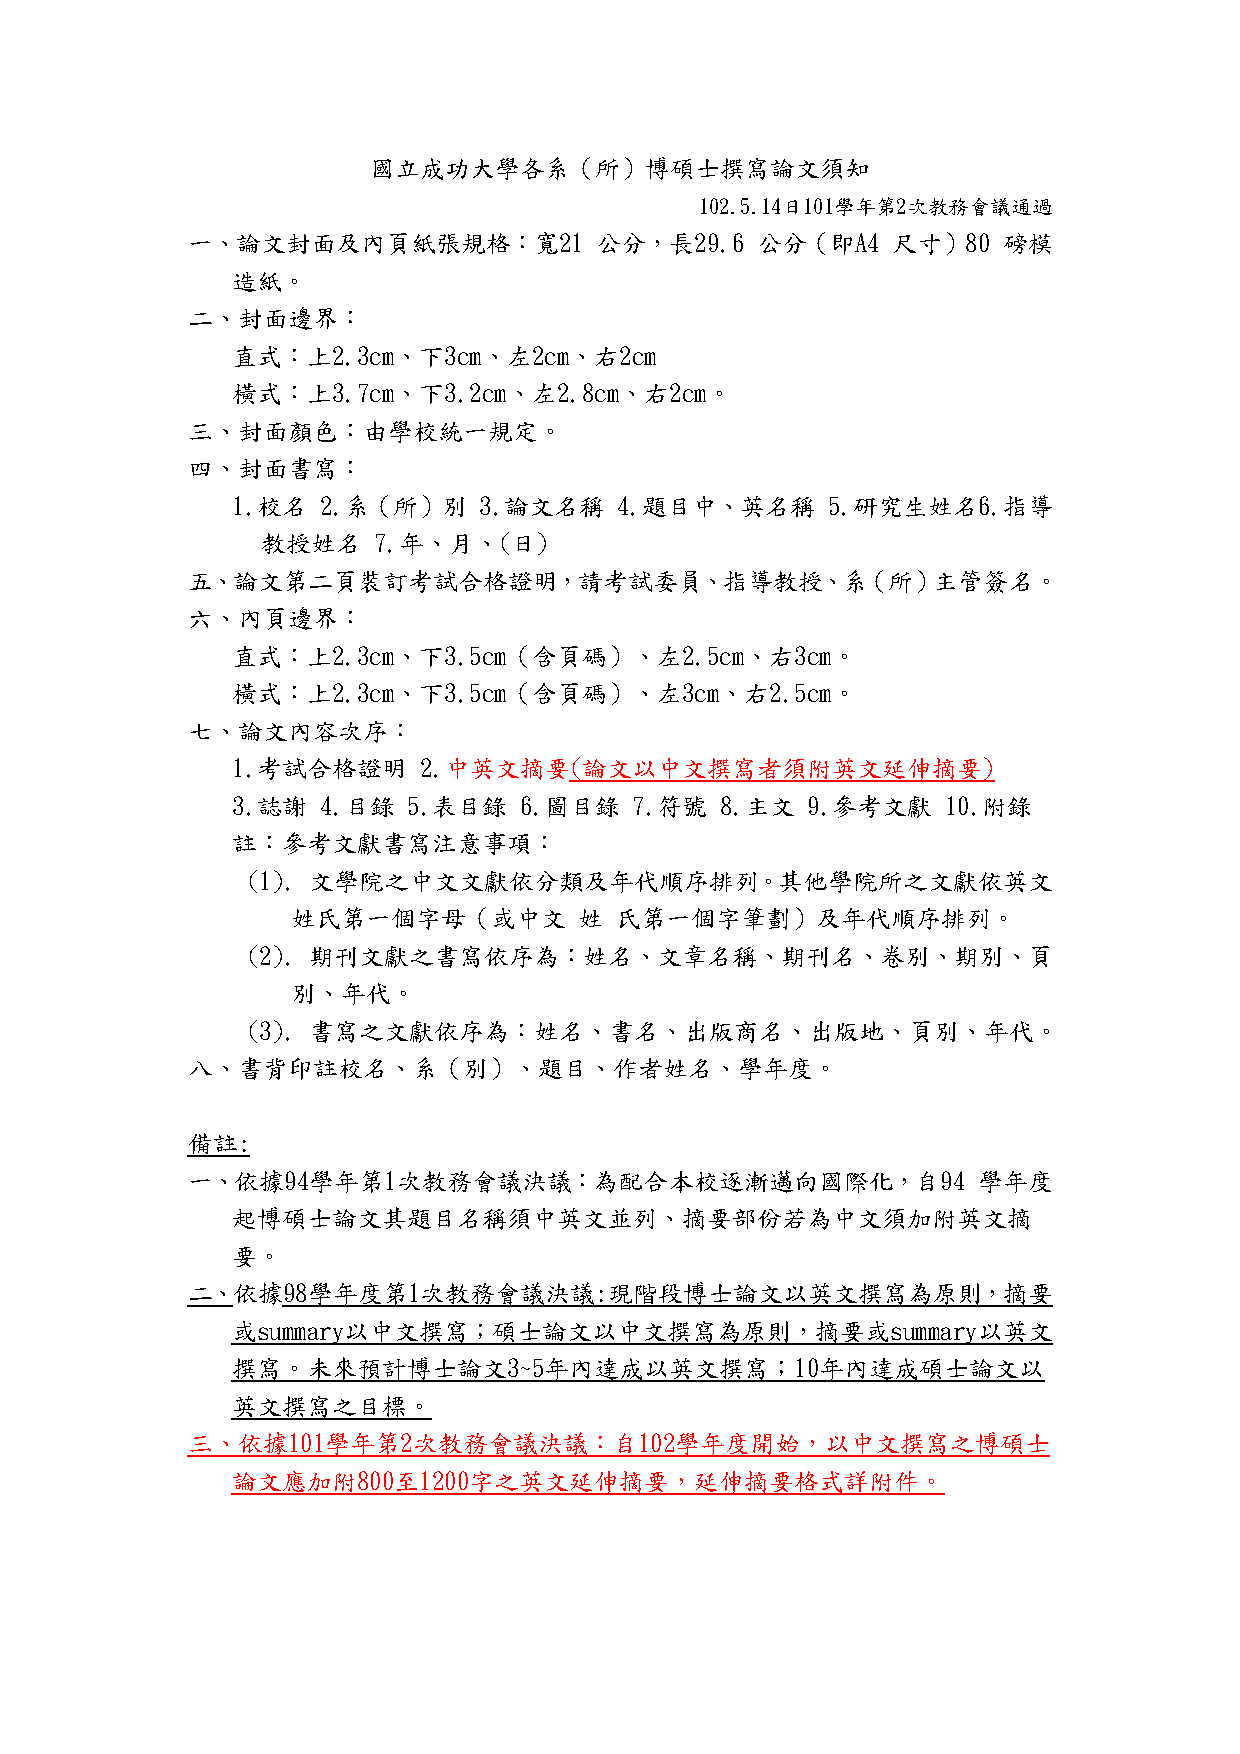
\includepdf[pages=-]{./example/appendix/pdf/thesis-spec.pdf}

% ------------------------------------------------
% End of page
% ------------------------------------------------
